This section describes how cache primitives can be applied to the context of work-sharing in large-scale distributed computing engines. The optimization process contains 4 phases and is described in Figure \ref{fig:phases_mqo}. Queries submitted by multiple users are parsed, analyzed and individually optimized by the query optimizer in normal way. Our optimization process starts with the optimized logical plan (the optimized operator tree) of each query as the input. In this paper, we are using the term \emph{logical plan} as the logical representation of a query. Those (optimized) logical plans are sent to a central server where our optimizations are applied.
\begin{figure}[!htb]
	\centering
 	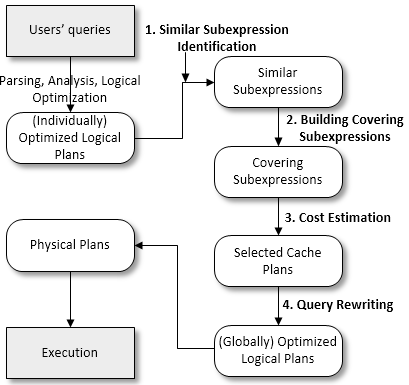
\includegraphics[scale=0.7]{figures/phases_mqo}
   	\caption{Proposed architecture.} 
   	\label{fig:phases_mqo}
\end{figure}

\textbf{Phase 1: Similar subExpressions(SEs) identification}\\
The goal of this phase is to quickly identify all potential sharing opportunities - the Similar Subexpressions (SEs). We compute an \emph{operator fingerprint} for each operator in each logical plan and store it in a fingerprint table. If two operators (and its descendants) have the same fingerprint then we call them similar subexpressions. We will discuss this technique in Section \ref{sec:common_sub}. Found similar subexpressions represents the potential candidates for building covering subexpressions (CEs) in the next phase.

\textbf{Phase 2: Building Covering SubExpressions}\\
Given the sets of SEs, the optimizer first tries to eliminate bad candidates for sharing with the help of cardinality and cost estimation. In this phase, some heuristics are applied to quickly reduce the solution space. Then for each set of SEs, we construct a CE that covers the computation of those expressions. Some CEs are dependent on other CEs, thus CEs are put into groups (classes). Some CEs might become \emph{cache plans} after the cost-based optimization in phase 3.

\textbf{Phase 3: Cost-based optimization}\\
This phase achieves the objective of selecting the best combination of CEs which then become \emph{cache plans}, taking into account the memory constraints and the cost of the caching operation. By using our cost estimation, each CE in previous phase will be assigned a weight and a profit. Finding the best \emph{cache plans} is the most important materialization of our idea to achieve high performance work sharing. We model the challenge such that solving it is equal to solving the Multiple Choice Knapsack problem.

\textbf{Phase 4: Query rewriting}\\
Finally, the input queries are rewritten in which the cache plans are employed. This step involves some basic query transformations on the original queries.

%%%%%%%%%%%%%%%%%%%%%%%%%%%%%%%%%%%%%%%%%%%%%%%%%%%%%%%%%%%%%%%%%%%%%%%%%%%%%%%
\subsection{Common subexpression identification}
\label{sec:common_sub}
The goal of this phase is to quickly identify all potential sharing opportunities in a query and among different queries. The input of this phase is a set of logical plans that are already parsed, analyzed and optimized individually. A logical plan is the internal form representing a query. It is a tree with nodes are logical operators supported by the execution engine. Each operator has its own attribute(s) (filter predicate, project columns, joining condition, etc.).

Our optimization process starts with the optimized logical plans (right before being transformed into physical plans) as the input. Note that we simplified the problem by only focusing on the locally optimal query plans that can derive globally better ones. The first reason is that all queries are already optimized by the same techniques (for example the rule-based optimizer) and usually, the selection and projection operators are pushed to the relations as close as possible. We want to quickly obtain and identify the potential sharing opportunities without paying too much the cost of taking into consideration each single generated logical plan for each query as in \cite{zhou2007efficient}. Keeping that in mind, it is the target of this step to quickly identify and produce reasonable good candidates.

We begin with finding the similar subexpressions in the trees. As being discussed in Section \ref{sec:problem}, we need to strike a balance between (low) memory utilization and (high) benefits from caching. Considering a query has only selection and projection operators, then the higher the node in that tree is, the more selective (less output data) it will be. In other words, some SEs can be safely eliminated from consideration because sharing (caching) them is always worse than some others. However, we may have multiple options if the tree contains one of the following operators: union, cartesian product and join. They are the operators that could possibly produce many output data, even more than the input. Such operators are classified into the \emph{cache-unfriendly operators} group. The rest are \emph{cache-friendly operators} (Filter, Project, Sort, Limit, etc.). Going back to the example in Section \ref{sec:problem}, because SE2, SE3 and SE4 contains only \emph{cache-friendly operators}, we stop looking at the smaller subexpressions for more sharing possibilities. SE1, however, has one \emph{cache-unfriendly operator} - Join. Then we can either select this candidate (SE1) or the 2 smaller ones (SE2 and SE3). We may not be able to immediately conclude which SE is better to share. It depends on multiple criteria (how much we can save in each case, how much data each produces and the memory available, etc.). Potential options are: $\{SE1, SE2, SE3, (SE2, SE3)\}$.

We use the \emph{operator fingerprints} as a technique to detect the similar subexpressions. We first describe how to compute it and how to produce only the ``good" SE candidates. The fingerprint $FP(u)$ of an operator $u$ is computed by:
\[FP(u)= h(H(u) | Sort(FP(u.lchild), FP(u.rchild))) (1)\]
where $h$ is a robust hash function (for example SHA256) and 
\[H(u)=
\begin{cases}
 & h(u.label),\ u= \{Filter, Project\}\\ 
 & h(u.label, u.attributes)),\ otherwise
\end{cases} (2)\]

Node $u$ in the operator tree has its label $u.label$ (operator name) and attributes $u.attributes$ (filter predicate, projection columns, joining conditions, etc.). The $Sort$ in (1) ensures the isomorphic property, for example $TableA\ JOIN\ TableB$ and $TableB\ JOIN\ TableA$ are two isomorphic expressions. If $u$ is a binary node, we have $u.lchild$ and $u.rchild$ as the left and right child. If $u$ is a unary node or a leaf node, (1) will become $FP(u)= h(H(u), FP(u.child))$ and $FP(u)= h(H(u))$ respectively. Note that the fingerprint of a node (an operator) is computed after computing fingerprint of its child(s). Two operators (and its descendants) have the same fingerprint then we call them similar subexpressions. They must have the same tree structure and property. Treating the Filter and Project operations differently in (2) allows us to identify SEs having different filtering predicates and projections. In phase 2, they can be transformed into equivalent expressions sharing a common subexpression. For instance $e1 = Filter_{a>10}(x)$ and $e2 = Filter_{b<30}(x)$ are similar subexpressions, then $e1, e2$ can be transformed into $Filter_{a>10}(Filter_{a>10\ \cup \ b < 30}(x))$ and $Filter_{b<30}(Filter_{a>10\ \cup \ b < 30}(x))$ without changing the expression's result.

Now that we have a mean to compare two operator trees, algorithm \ref{sec:common_sub_alg} searches for SEs among a set of trees while avoid producing worse candidates.

\begin{algorithm}
	\caption{Build hash tree}\label{sec:buildht_alg}
	Input: a logical plans (tree)\\
	Output: HashMap[node, fingerprint]
	\begin{algorithmic}[1]
		\Procedure{$BuildHashTree([T])$}{}
		\State $HT:\{(node, fingerprint)\}=$ empty hash tree
		\For{each node $u$ in $T$}
			\State compute fingerprint $opFT$ for $u$ using (1) and (2)
			\State put $(u, opFT)$ into $HT$
		\EndFor
		\State \Return  $HT$
		\EndProcedure
	\end{algorithmic}
\end{algorithm}

\begin{algorithm}
\caption{Identify similar subexpressions}\label{sec:common_sub_alg}
Input: Array of logical plans (trees)\\
Output: List of SEs put together in group
\begin{algorithmic}[1]
\Procedure{$IdentifySEs([T_{1}, T_{2}, ... T_{N}])$}{}
\State $FT:\{(fp, [nodes])\} =$ empty fingerprint table
%\State $common\_sub\_expressions = \{\}$
\For{each tree $T_{i}, i = 1..N$}
	\State$HT(i) = BuildHashTree(T_{i})$
	\State $AllowedMatching = True$	
	\For{each node $u$ in $T_{i}$ follow the DFS traversal}
		\State $opFP = HT(i)(u)$
		\State $IsMatched = FT$ contains $opFP$
		\If {$AllowedMatching$}
				\State Add $(opFP, u)$ entry to $FT$
		\EndIf
		\State $AllowedMatching = True$	
		\If {$IsMatched$ $AND$ the tree rooted at u does not has cache-unfriendly operator}
			\State Stop the search on u's descendants
		\ElsIf {$IsMatched$ $AND$ the tree rooted at u has cache-unfriendly operator $AND$ $u$ is cache-friendly operator}
			\State $AllowedMatching = False$	
		\EndIf		
	\EndFor
	
\EndFor
\State remove any entries (fp, [nodes]) in FT that has length(nodes) = 1
\State \Return  $FT$
\EndProcedure
\end{algorithmic}
\end{algorithm}

By using the expression (1) and (2), algorithm \ref{sec:buildht_alg} builds a HashTree for each input tree (line 4) of algorithm \ref{sec:common_sub_alg}. Algorithm \ref{sec:buildht_alg} just shows the simplified pseudo code. (Dynamic programming can be applied to save the computations in the for loop). A single fingerprint table (line 2) is used for tracking the matches. Trees with the same fingerprint (same key) will be put in the same group. Following the depth-first-search, each tree and its \emph{operator fingerprint} are added to the fingerprint table (line 10). As being discussed, if we encounter a match on a tree having only cache-friendly operators, then we can safely skip the search on the descendants (line 13 and 14). A group of SEs is detected whenever that group has 2 or more SEs (line 20). Algorithm \ref{sec:common_sub_alg} has O(N*M) complexity where N is the number of trees and M is the average number of nodes per tree.
%%%%%%%%%%%%%%%%%%%%%%%%%%%%%%%%%%%%%%%%%%%%%%%%%%%%%%%%%%%%%%%%%%%%%%%%%%%%%%%

%%%%%%%%%%%%%%%%%%%%%%%%%%%%%%%%%%%%%%%%%%%%%%%%%%%%%%%%%%%%%%%%%%%%%%%%%%%%%%%
\subsection{Building Covering SubExpression}
\label{sec:covering_subexpression}
We identified the potential sharing candidates (SEs) from the input queries, it is the goal of this phase to build the covering subexpressions (CEs) that are the ``covering" computations. Given the sets of SEs, the optimizer first tries to eliminate obviously bad candidates for sharing with the help of cardinality and cost estimation described in Section \ref{sec:cardinality}. Then for each set of SEs, we construct a single CE to produce all common sharing tuples for the consumers (all SEs in that set). Some CEs might become \emph{cache plans} after the cost-based optimization in phase 3. 

In this paper, we define the \emph{cache plan} as the materialization for our work sharing idea. A \emph{cache plan} is a CE defining the result of a materialized view. In other words, cache plans can be seen as temporary views in RDBMSes and to be materialized in RAM. In our work, \emph{cache plans} (selected CEs) will be executed only once and the result is materialized in RAM so that it could be reused multiple times to achieve work sharing. When a query executes, the engine searches in the distributed memory cache to determine whether the results already exists. If yes, it retrieves the result instead. If no, it executes, return the results as output and store them back to the memory cache.

To simplify the problem, we consider the case where only one group of n SEs was identified among the input queries. That means a CE can be built to cover those expressions. We first compare the cost between two approaches: with and without our optimization. We use the notation $C_{E}^{se}$ and $C_{E}^{ce}$ to denote the executing costs of SE $se$ and CE $ce$. $C_{W}^{ce}$ and $C_{R}^{ce}$ are the costs of materializing (writing) the result of CE $ce$ to RAM and retrieving (reading) it back. $C_{COMP}^{se}$ indicates the cost of using the CE to answer the SE $se$.

Given a group of n SEs detected in phase 1, the cost of executing them without optimization can be computed by summing all individual executing costs: $C = \sum _{i=1}^{n}C_{E}^{se_i}$. In contrast, by building a CE and use it as a \emph{cache plan}, this cost becomes: 
$C^* = C_{E}^{ce} + C_{W}^{ce} + \sum _{i=1}^{n}(C_{R}^{ce} + C_{COMP}^{se_i})$. 
CE will be executed and materialized to RAM once. Then the result is read back to answer each individual SE. Only when $C^* < C$, caching brings some benefit in reducing the total job's running time. $C_{E}^{se}$, $C_{E}^{ce}$ and $C_{COMP}^{se_i}$ can be estimated by using cost estimation. $C_{W}^{ce}$ is proportional to the cache size of $ce$, which can be estimated using cardinality estimation. $C_{R}^{ce}$, the cost of reading the cached result of $ce$, is expected to be relatively small. We define the profit $P = (C^*-C)$ which is the profit of using a $ce$ as the cache plan.

%%%%%%%%%%%%%%%%%%%%%%%%%%%%%%%%%%%%%%%%%%%%%%%%%%%%%%%%%%%%%%%%%%%%%%%%%%%%%%%
\subsubsection{CE construction}
\label{sec:ce-construction}
A CE will be built for each group of SEs. Obviously, for SEs that are actually identical expressions, the CE to be built is exactly the same as the SE. Otherwise, we have to apply some transformations on the SEs. The CE is constructed top-down by OR-ing the filtering predicates and combining the projection columns in the SEs. By doing so, the CE could ``cover'' all records required by its consumers. We also remove duplicated predicates to simplify the operators. Figure \ref{fig:covering} illustrates an example of building the covering subexpression for 2 simple SEs. Traversing top-down 2 trees at the same time, whenever projection or filering operators are encountered, we combine their attributes.

\begin{figure}[!htb]
	\centering
	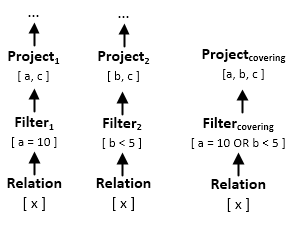
\includegraphics[scale=0.75]{figures/covering}
	\caption{Building covering subexpression example. The first and second trees are two SEs. The third tree is the CE}
	\label{fig:covering}
\end{figure}
%%%%%%%%%%%%%%%%%%%%%%%%%%%%%%%%%%%%%%%%%%%%%%%%%%%%%%%%%%%%%%%%%%%%%%%%%%%%%%%


%%%%%%%%%%%%%%%%%%%%%%%%%%%%%%%%%%%%%%%%%%%%%%%%%%%%%%%%%%%%%%%%%%%%%%%%%%%%%%%
\subsubsection{Pruning bad SEs}
\label{sec:se-prune}
The size of the \emph{cache plans} not only affects the memory occupation but also brings materializing costs. Intuitively, good candidates of \emph{cache plans} are those satisfy the memory constraint while (1) have high frequent of use and/or (2) are expensive to (re)compute, for example producing small amount of output while reading and computing a large amount of input data. Thus, cheap SEs (fast to compute) and heavy SEs (their output exceeds the memory constraint) should be eliminated early from consideration of building the CE. We rather compute them from scratch than just gain a small benefit while paying a big cost in caching a large amount of data. The cost and cardinality estimation we propose in the next section is used to estimate the execution cost and output size of a query.

%%%%%%%%%%%%%%%%%%%%%%%%%%%%%%%%%%%%%%%%%%%%%%%%%%%%%%%%%%%%%%%%%%%%%%%%%%%%%%%
%%%%%%%%%%%%%%%%%%%%%%%%%%%%%%%%%%%%%%%%%%%%%%%%%%%%%%%%%%%%%%%%%%%%%%%%%%%%%%%

%%%%%%%%%%%%%%%%%%%%%%%%%%%%%%%%%%%%%%%%%%%%%%%%%%%%%%%%%%%%%%%%%%%%%%%%%%%%%%%
\subsection{Cost-based optimization}
\label{sec:cbo}
%%%%%%%%%%%%%%%%%%%%%%%%%%%%%%%%%%%%%%%%%%%%%%%%%%%%%%%%%%%%%%%%%%%%%%%%%%%%%%%
\subsubsection{Cardinality and cost estimation}
\label{sec:cardinality}
We design a cardinality and cost estimator to estimate the query's output size and execution cost. Just as traditional work, the system analyzes relational operators and uses some pre-computed statistics data of the input tables.

Computing the query's output size mainly relies on the statistics data, which are computed in 2 levels: relation and column. In relation level, the system obtains the number of records and average record size. In more detail level - column, the system collects the min, max, the cardinality and builds an equi-width histogram for each column. The output size of each operator is estimated under the uniform distribution assumption. 

Although simple, we just want a good estimation to avoid obviously bad plans. More complex histogram techniques could be used to improve the estimation accuracy.


We focus on the CPU, disk I/O and network costs in estimating the total execution cost of a query because they are the three most dominant ones. Those costs are the results of the multiplication between the pre-defined constants and the estimated number of records.




%%%%%%%%%%%%%%%%%%%%%%%%%%%%%%%%%%%%%%%%%%%%%%%%%%%%%%%%%%%%%%%%%%%%%%%%%%%%%%%


%%%%%%%%%%%%%%%%%%%%%%%%%%%%%%%%%%%%%%%%%%%%%%%%%%%%%%%%%%%%%%%%%%%%%%%%%%%%%%%
\subsubsection{Cache plans selection}
\label{sec:cbo-o}
Our problem is to select the best combination of CEs to form the \emph{cache plans}. For each \emph{cache plan}, we compute the (profit, weight). Let's call $W$ is the total cache capacity of the cluster. Then our optimization problem is to maximize the $\sum profit$ under a limited memory capacity: $\sum weight \leq W$. This is the knapsack problem and could be solved by many approaches \cite{•}.

The weight is estimated thanks to the cardinality estimation in section \ref{sec:cardinality}. The profit is the cost difference between (1) executing $n$ SEs and (2) executing the \emph{cache plan} and reused in multiple places. The cost of executing individual SEs are $\sum_{i=1}^n SE_i$ apparently. On the other hand, the cost of (2) is the cost of executing the \emph{cache plan} once, materializing the result to RAM and n times * retrieving the cached data. Furthermore, the cost of applying the \emph{extraction plans} in section \ref{sec:query_rewriting} to compensate the CE and the garbage collection effect are also parts of (2).

Then the combination of \emph{cache plans} to maximize the benefit under the memory limit is equivalent to solving the knapsack problem. Thus, we will be able to first select the best CE among different sharing options.
%%%%%%%%%%%%%%%%%%%%%%%%%%%%%%%%%%%%%%%%%%%%%%%%%%%%%%%%%%%%%%%%%%%%%%%%%%%%%%%

%%%%%%%%%%%%%%%%%%%%%%%%%%%%%%%%%%%%%%%%%%%%%%%%%%%%%%%%%%%%%%%%%%%%%%%%%%%%%%%

%%%%%%%%%%%%%%%%%%%%%%%%%%%%%%%%%%%%%%%%%%%%%%%%%%%%%%%%%%%%%%%%%%%%%%%%%%%%%%%
\subsection{Query Rewriting}
\label{sec:query_rewriting}
Now that we selected the best combination of \emph{cache plans}, the last step is to transform the original input queries to use them. First, the execution engine should be noticed that the output of \emph{cache plans} will be materialized in RAM after its execution. Next, the transformation applied on the input queries is the replacement of SEs by the \emph{extraction plans} on top of the \emph{cache plans}. Remember that \emph{cache plans} are the selected covering subexpressions that covers the records for their consumers. We need to re-apply the filtering and projection to assures the output of queries does not change.

For each input query having the SE and employing the cache plan respectively, we build an \emph{extraction plan} that compensates the cache plan such that the output of the extraction plan on top of the cache plan is equals to the output of that SE. The query rewriting in Figure \ref{fig:rewrite} is a simple example illustrating the technique. In more abstract, we build the \emph{extraction plans} by AND-ing the filtering predicates and combining the top projection columns of the SE.

\begin{figure}[!htb]
	\centering
ubstaint	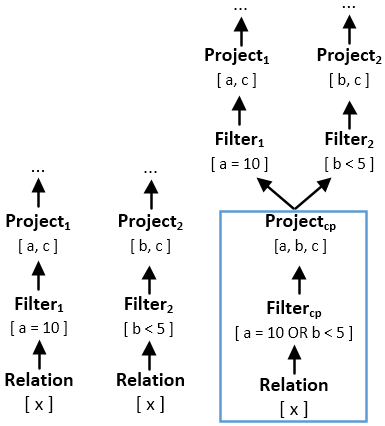
\includegraphics[scale=0.55]{figures/rewrite}
	\caption{Query rewriting example. The tree in rectangle is the cache plan}
   	\label{fig:rewrite}
\end{figure}
%%%%%%%%%%%%%%%%%%%%%%%%%%%%%%%%%%%%%%%%%%%%%%%%%%%%%%%%%%%%%%%%%%%%%%%%%%%%%%%

We next cover in detail the implementation of our system running on Apache Spark and Spark SQL.